\documentclass{article}
\usepackage[UTF8]{ctex}
\usepackage{geometry}
\usepackage{natbib}
\usepackage{url}
\usepackage{graphicx}
\usepackage{subfigure}
\usepackage{enumerate}
\geometry{left=3.18cm,right=3.18cm,top=2.54cm,bottom=2.54cm}
\usepackage{graphicx}
\pagestyle{plain}	
\usepackage{setspace}
\usepackage{indentfirst}
\usepackage{caption2}
\usepackage{datetime} %日期
\renewcommand{\today}{\number\year 年 \number\month 月 \number\day 日}
\renewcommand{\captionlabelfont}{\small}
\renewcommand{\captionfont}{\small}
\setlength{\parindent}{2em}
\begin{document}

\begin{figure}
    \centering
    
\includegraphics[width=8cm]{upc.png}

    \label{figupc}
\end{figure}

	\begin{center}
		\quad \\
		\quad \\
		\heiti \fontsize{45}{17} \quad \quad \quad 
		\vskip 1.5cm
		\heiti \zihao{2} 《计算科学导论》课程总结报告
	\end{center}
	\vskip 2.0cm
		
	\begin{quotation}
% 	\begin{center}
		\doublespacing
		
        \zihao{4}\par\setlength\parindent{7em}
		\quad 

		学生姓名:\underline{\qquad  张世琛 \qquad \qquad}

		学\hspace{0.61cm} 号:\underline{\qquad 1804030401\qquad}
		
		专业班级:\underline{\qquad 计科1802 \qquad  }
		
        学\hspace{0.61cm} 院:\underline{计算机科学与技术学院}
% 	\end{center}
		\vskip 2cm
		\centering
		\begin{table}[h]
            \centering 
            \zihao{4}
            \begin{tabular}{|c|c|c|c|c|c|c|}
            % 这里的rl 与表格对应可以看到,姓名是r,右对齐的;学号是l,左对齐的;若想居中,使用c关键字。
                \hline
                课程认识 & 问题思 考 & 格式规范  & IT工具  & Latex附加  & 总分 & 评阅教师 \\
                30\% & 30\% & 20\% & 20\% & 10\% &  &  \\
                \hline
                 & & & & & &\\
                & & & & & &\\
                \hline
            \end{tabular}
        \end{table}
		\vskip 2cm
		\today
	\end{quotation}

\thispagestyle{empty}
\newpage
\setcounter{page}{1}
% 在这之前是封面,在这之后是正文
\section{引言}
    这个学期,我们学习了《计算机科学导论》这门课,通过这门课课程的学习,我对计算机科学这一门学科了解了很多,从比较科学的角度去认识和学习的计算机科学。因此,学习了这门课,我对自己选修的这个专业有了很大程度上的认识。不再像大一时还没有学习这门课程前的那样子了,那时候对自己所学习的东西一点也不了解,也不知道该用怎么样的方法去学习专业的课程。总的来说,有了不小的收获。对于我们学好计算机科学,顺利完成学业,有很大的帮助。这门课的开始,我们首先学习了计算科学的含义,来历等问题,从比较哲学化的角度向我们阐述了这门科学!我认识到了计算科学的内涵有狭义和广义之分,狭义方面指的是我们所研究的计算机科学与技术,是对计算机问题的一般研究。广义的计算科学包含的内容要广得多,它不仅涵盖了计算机科学与技术的研究范畴,而且还包含了图形学与图像处理、数据库系统、人工智能和虚拟现实等更多的内涵。随后我们学习了计算科学的基本概念和基本知识,还有计算科学的意义,内容和方法,最后我还学习了如何计算科学这门学科。在第四章的学习中,让我明白了学习这门学科的方法,让我知道了我学习的这个专业所走的一个方向,以及这个专业的培养规格和目标,还有它的课程体系,以及教学计划。让我知道自己提高专业技术能力的途径与方法。
\section{对计算科学导论这门课程的认识、体会}
首先,计算机科学导论这门课是让我们对这计算机这个学科有所了解,为我们的专业学习打好基础,这样我们才能更好地学习这个专业。它从如何引导我们成长为一个优秀的专业技术人员这样一个问题谈起,从一个更一般的认识层面上掌握如何学习一门专业知识的方式方法,解决如何认识计算机科学与技术,如何学习计算机科学与技术的问题。这门课程从计算机这一领域出发,谈到了计算科学的基本知识,计算科学的意义、内容和方法。其中包括计算模型与二进制,通用数字计算机系统结构与工作原理,数字逻辑与集成电路,机器指令与汇编语言,算法、过程与程序,高级语言与程序设计,系统软件与应用软件,计算机组织与体系结构,并行计算机、通道与并行计算,计算机网络与通信,计算机图形学与图像处理,逻辑与人工智能到数据处理与演化计,计算机科学与技术一级学科等领域内的一些重要的基本概念。还有,它所阐述的理论和方法对于我们今后的学习起到一个指导作用。它教会我们怎样才是一个科学的思维过程,面对所要处理和解决的问题,我们要有一套怎样的科学细想方法:一个科学的认识,一套科学的方法,一个科学的程序。看问题要从本质出发,发现问题的根本所在,这样给有利于实际问题的解决。强调了理论知识的重要性,这也是这门学科与其它学科的明显区别。在这个学期的课程中,我学习了数据结构,它的重要性不言而喻了,学完数据结构你会对你的编程思想进行一番革命性的洗礼,会对如何建立一个合理高效的算法有一个清楚的认识。例如说对于数据结扎中算法的建立我想大家应当注意以下几点:当遇到一个算法问题时,首先要知道自己以前有没有处理过这种问题.如果见过,那么你一般会顺利地做出来;如果没见过,那么考虑以下问题:
\begin{enumerate}[(1)]  
    \item 问题所要求编写的算法属于哪种类型?(如建立数据结构,修改数据结构,遍历,  
    \item 继续分析问题的数学本质.根据你以前的编程经验,设想一种可能是可行的解决办法。
    \item 确认你的思路可行以后,开始编写程序.在编写代码的过程中,尽可能把各种问题考虑得详细,周密.程序应该具有良好的结构,并且在关键的地方配有注释.
    \item 举一个例子,然后在纸上用笔执行你的程序,进一步验证其正确性.当遇到与你的设想不符的情况时,分析问题产生的原因是编程方面的问题还是算法思想本身有问题.要有丰富的想象力,就是说当一条路走不通时,不要钻牛角尖,要敢于推翻自己的想法.
\end{enumerate}

有了这一理论上的认识,根据其结构特点,思考实现这一问题的算法,之后才进行实践编程。通过这门课程的学习,使我能从多方面分析,不但明白了该门课程的重要性,让我更加重视这数据结构这门课,还让我对怎么样去学习这门课有了更加深  的认识。还有,在学习计算机科学导论这门课的时候,老师反反复复地提到了要我们重视打好基础的重要性,还提到了很多有关她自己在计算机学科上面所经历的事情,还引导我们怎么学习自己的课程。

对计算机来说,我个人最大的认识就是:从原来的仅仅认为它是一台机器到现在知道它是一门庞大的学科!计算机这一行业发展起来至今天的普遍应用只有短短的几十年。从稀有到普及,这一领域的发展可以说是二十世纪到二十一世纪发展最迅猛的领域之一。而且,它还是社会发展进程中依赖比重很大的一门学科。在生活中更少不了它的使用。所以,学习计算机技术的重要性就显得尤为突出了。并且,大学生将会是未来社会中技术运用者的主力军。那么,对于我们计算机技术水平和能力的要求,就相对的要高了。我们学计算机,至少具备下面的能力:懂得计算机基本方法。具备较强数据库安装调试与简单开发能力。掌握信息管理系统的应用、开发及维护技术。具有计算机网络系统的设计、安装、调试、管理能力,并且掌握计算机网络环境下的计算机信息管理系统开发的基本方法和维护技能。当然,不同专业对应着不同的能力要求。对于初学者的我来说 ,以上的计算机基础能力要求我尚且未能达到,但我相信在大学的四年中可以使自身的能力上升一个高度。和很多同学一样,我以前对计算机的了解相当少,刚开始认识计算机是从感性上来认识计算机这一门学科的,开始时只是简单的对它有一个大致的印象。经过一个学期的短暂学习,进一步的能从理性的角度去深入认识它。计算机科学与技术是研究计算机的设计与制造和利用计算机进行信息获取、表示、存储、处理、控制等的理论、原则、方法和技术的学科,包含科学与技术两方面。科学这一方面主要是研究现象、揭示规律;技术则是研究计算机和研究使用计算机进行信息处理的方法和技术手段。所以,技术和科学相辅相成,两者的融合构成了这一学科。对于学习计算机科学与技术,大家都知道两个是不能简单的将之分开为计算机科学和计算机技术来学习或者讨论--至少,在本科阶段不能将其切分开来。因为计算机科学是以理论为基础的,它需要大量的实践去验证,而实践需要技术,两者相辅相成。从本质上了来讲,计算机科学与技术,它是一门科学性与工程性并重的学科,表现出了它理论性和实践性紧密结合的特征。这也是为什么我们学生不能将其分开成科学和技术来学习的原因。在大一期间,趁着时间比较宽裕,自身发展空间较大,先进行此学科的概括性了解,为以后的深入学习打下基础。上升到大二时期,是进行不断充实的时期。在这一时期,深入研究计算机知识,更多的去理解系统原理,数据结构,特别是要打下牢靠的编程基础,培养自己的基本能力,强化自身的理论基础。大三时期,注重培养自己的创新能力,将理论和技术运用到自己的想法当中去,给自己锻炼的机会,真正达到学以致用。到最后,则是培养自己的实践能力(比如说创业或者进入公司实习培养自己的“实战能力”),从运用中理解计算机科学与技术。

根据自身的实际情况和结合自己的专业方向,我更感兴趣于程序语言能力的培养。程序语言是大学学习的重要内容之一,而学习此门课程也得注意到一个问题,那就是程序设计语言的更新速度相当快。如何才能学好程序设计语言也是个需要解决的问题。以后的工作也很大可能性上是与计算机有关。所以,在大学四年中,在修习数学和外语的基础上,我将会将自己的研究方向朝向培养程序语言能力的领域(我更热衷于这个)。 
\par
\subsection{算法的概念和认识}
通过阅读《算法导论》\citep{suanfadaolun2006}从广义上理解,算法是解决一个问题的方法和步骤。狭义上特指能够在计算机上实现和分析的计算机算法。算法是一组明确的、可执行步骤的有序集合,在有限的时间内终止并产生结果。算法就是被精确定义的一组规则,也可以说算法是有限的、有序的、有效的计算机指令的集合。不同的问题需要不同的算法来解决,同一个问题也可能存在不同的算法。但总的来说,它应有以下特征:有穷行、确定性、可行性、输入数据与输出数据的要求。有穷性是指一个算法必须在有限的操作步骤内以及合理的时间内执行完成;确定性是指算法中的每一个步骤都必须有明确的含义,不允许存在二义性;有效性是指算法中每一个步骤必须能够实现而且执行的结果能够达到预期的目的,实现预定的功能。输入数据与输出数据的要求是指一个算法应该有0个或多个输入数据、有一个或多个输出数据。常用算法有递归算法、迭代算法、穷举算法、贪婪算法。

在学习过程中,要求我们设计一个算法在满足前面几个特性的同时,应将算法的健壮性考虑进去,因为评价一个算法的优劣,不仅看它的正确性、可理解性,还要看它的健壮性。在程序中考虑算法的健壮性就显得相当必要了。在练习编程序的时候,老师也注重看我们所编程序中的算法的好与差,这样无形当中就培养了我们在设计一个算法的分析和统筹能力。而在计算机软件系统中,算法的设计与分析处于核心地位。这就显得尤为重要了。一个算法从开始到完全显现,设计与分析就相当于整个工程中的主干。两者是相互依存的,设计出的算法需要检验和评价,对算法的分析反过来又将改进算法。我认为,一个好的算法是程序的灵魂。举个例子,在后续使用中,程序运行过程中很有可能会出现输入数据的偏差,那么,好的算法必定会有较好的容错性即健壮性。它的好处还在于可以减少后面软件的维修成本。是比软件开发成本高出很多的。 
\subsection{卷积神经网络}
卷积神经网络(Convolutional Neural Networks, CNN)是一类包含卷积计算且具有深度结构的前馈神经网络(Feedforward Neural Networks),是深度学习(deep learning)的代表算法之一。

卷积神经网络具有表征学习(representation learning)能力,能够按其阶层结构对输入信息进行平移不变分类(shift-invariant classification),因此也被称为“平移不变人工神经网络(Shift-Invariant Artificial Neural Networks, SIANN)”。
对卷积神经网络的研究始于二十世纪80至90年代,时间延迟网络和LeNet-5是最早出现的卷积神经网络 [4]  ;在二十一世纪后,随着深度学习理论的提出和数值计算设备的改进,卷积神经网络得到了快速发展,并被应用于计算机视觉、自然语言处理等领域。
\begin{figure}[h!]
                \centering
                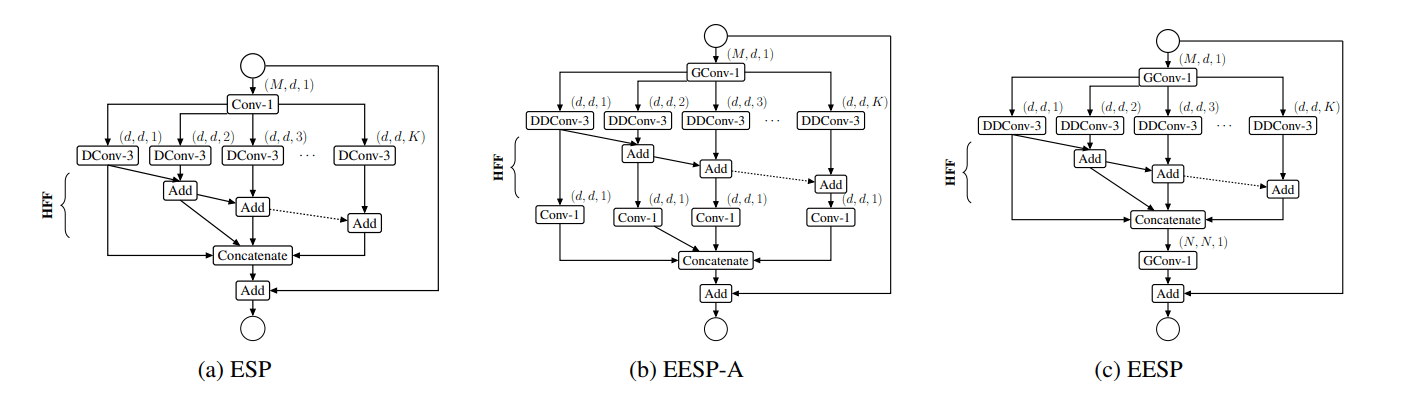
\includegraphics[width=12.5cm,height=5.5cm]{8.png}
                \caption{卷积神经网络}
                \label{fig:universe}
            \end{figure}
卷积神经网络仿造生物的视知觉(visual perception)机制构建,可以进行监督学习和非监督学习,其隐含层内的卷积核参数共享和层间连接的稀疏性使得卷积神经网络能够以较小的计算量对格点化(grid-like topology)特征,例如像素和音频进行学习、有稳定的效果且对数据没有额外的特征工程(feature engineering)要求。
\subsection{信息安全}
信息安全是指信息网络的硬件、软件及其系统中的数据受到保护,不受偶然的或者恶意的原因而遭到破坏、更改、泄露,系统连续可靠地运行,信息服务不中断。信息安全主要包括以下五个方面的内容,即需保证信息的保密性、真实性、完整性、未授权拷贝和所寄生系统的安全性。其根本目的就是使内部的信息不受外部的威胁,因此信息通常要加密。信息安全是一门设计算机科学、网络技术、通信技术、密码技术、信息安全技术、应用数学、数论、信息论等多种学科的综和性学科。信息安全的威胁主要有以下几方面: 

\begin{enumerate}[(1)]  
    \item 信息泄露:保护的信息被泄露或透露给某个非授权实体。   
    \item 破坏信息的完整性:数据被非授权地增删、修改或破坏而受到损失。
    \item 拒绝服务:信息使用者对信息或其他资源的合法访问被无条件的拒绝。 
    \item 非法使用(非授权访问):某一资源在未授权的情况下被使用。
    \item 窃听: 用各种可能的合法或非法的手段窃取系统的信息资源和敏感信息。
    \item 计算机病毒:计算机系统中实现传染和侵害功能的程序。
\end{enumerate}

现代信息技术的急剧发展造就了当前海量信息的不安全性,在这种情况下,信息安全就应运而生。我们知道,信息安全这一领域起步较晚(这是必然的,信息安全性问题在信息量越来越多之后才日益显现出来),现在实现信息安全的途径靠的是先进的技术以及严格的安全管理,法律约束和安全教育。对于信息安全这一行业,个人认为我们更应注重的是职业修养。在这一领域掌握着先进技术的人,不仅可以充当保护者的身份,反过来也会变成刺客。相对于某些国家来说,我国的技术水平较低,并且信息安全这一块起步也很晚,想要在以后的发展中处于有利地位,就需要发展起以我国国情为基础的信息安全工程,加强安全管理队伍的建设,制定出更加完善的网络安全管理体系。通过规范化的管理并结合先进技术的运用,使自身的网络更加的安全,创造出更舒适的网络环境,使得我国的网络事业能较好的发展起来。
\section{大数据人工智能网络技术中的应用}
人工智能\citep{AI}在计算机网络技术中的应用,作为计算机网络技术发展的必然趋势,这一技术的迅速普及和应用,对于计算机网络技术的安全管理、信息查询、智能化系统开发、环境支撑等功能的提升,同样发挥着积极的促进作用。
\subsection{增强网络信息的安全性}
人类社会进入大数据时代后,网络与人们日常生活的联系也越来越密切。然而由于网络在实际应用的过程中,存在着个人信息被恶意盗取、钱财被骗等各种各样的安全隐患。因此,怎样发挥人工智能技术的优势,提高网络信息的安全性,是当前社会各界广泛关注的焦点。人工智能与人们生活、工作、学习之间联系的日益密切,为社会的发展指明了方向。就目前而言,人工智能尚处于初期探索和应用的阶段,再加上相关安全防护的内容和措施还不完善,所以还无法进行大范围的推广和应用。如果计算机网络技术应用人工智能后,受到了恶意攻击后,人工智能失去控制的话,那么其所产生的后果是人类无法控制的,所以相关的科研人员必须严格的按照要求,控制好可能出现的安全隐患,为未来人工智能的全面推广和应用做好充分的准备。
\subsection{应用于网络管理与评级体系建设}
随着网络信息时代的来临,人们的不管是生活、工作还是学习已经离不开计算机的支持和帮助,为了最大限度的满足社会发展的要求,研究人员应该充分借助人工智能技术,积极的进行数据库的研发。借助人工智能技术,优化和完善现有数据库资源的功能,以便于为人们提供更加优质和全面的服务。此外,研究人员应该借助人工智能技术,及时的升级和优化现有网络系统,促进网络系统评级测试精确性的有效提升,同时也有助于研究人员及时的发现和解决网络系统中存在的各种安全隐患,确保网络系统的安全稳定运行。
\subsection{实现人工智能代理管理}
人工智能代理管理技术的推广和应用,为人们的生活提供了更大的便利和帮助。这里所说的人工智能代理管理实际上指的就是人工智能Agent技术,该技术作为一种全新的软件设备,主要是根据Agent知识库运行的特点,在全面分析处理网络信息的基础上,完成数据信息的处理工作。计算机网络用户在日常工作的过程中,运用这一技术进行网络数据信息的自定义,即可通过人工智能代理管理搜索和使用符合自身要求的数据信息,并将数据信息传输至用户指定的位置。例如,用户在搜索相关数据信息时,人工智能技管理中需要综合用户的各种需要,进行自动搜索,这种智能化、人性化的服务模式,不仅节省了用户搜索数据信息的时间和精力,同时也使用户切实的感受到了人工智能带来的优越性。
\section{进一步的思考}
\subsection{Java语言入门与进阶}
        《Java编程思想》\citep{java}
        基础语法,面向对象的特性及常用类

        集合,多线程,流对象,网络编程
\subsection{JavaWeb} 
       关系型数据库MySQL学习,以及用JDBC相关工具操作数据库

       前端知识学习,html,css,javascript,框架学习,bootstrap,jQuery等

       Web核心知识三大组件:servlet,filter,listener
       Linux及Nginx的学习
 \subsection{框架学习} 
      SSM框架学习,Mybatis,Spring,SpringMVC

       学习了解,NOSQL数据库redis,关系型数据库Oracle,Maven项目管理工具

       深入学习Spring家族,如Spring Data、Spring Boot、Spring Cloud等等
 \subsection{框架学习内功进阶} 
      JVM虚拟机,数据库优化,算法加强。

       阅读java源代码,如hashMap实现机制,垃圾回收实现机制,厚积薄发

       图像处理,机器学习,算法进阶,大数据开发,深度学习
  \subsection{什么是Servlet?} 
Servlet是运行在服务器端的Java应用程序,通俗地讲就是一个Java接口(java类),他能被服务器识别

实现该接口的类可以用来处理请求和发送响应,因此可以与数据库进行交互、响应客户请求,生成动态的Web资源。

它与传统java应用程序的区别是它是服务器和客户端之间的桥梁。

Servlet一般用于后台代码开发,用来调用DAO或者业务逻辑层来完成数据库操作,还可以用来接收表单参数和完成页面跳转。

\subsection{Filter:过滤器 } 
生活中的过滤器:净水器,空气净化器

  web中的过滤器:当访问服务器的资源时,过滤器可以将请求拦截下来,完成一些特殊的功能。

  过滤器的作用:
    一般用于完成通用的操作。如:登录验证、统一编码处理、敏感字符过滤.
\subsection{快速入门} 
  1. 步骤:
    \begin{itemize}

    \item 定义一个类,实现接口Filter
    \item 复写方法
    \item 配置拦截路径
    \begin{itemize}
    \item web.xml 
    \item 注解
    \end{itemize}
  \end{itemize}

  2. 过滤器执行流程
      \begin{itemize}
    \item 执行过滤器
    \item 执行放行后的资源
    \item 回来执行过滤器放行代码下边的代码
    \end{itemize}

  3. 过滤器生命周期方法
      \begin{itemize}
    \item init:在服务器启动后,会创建Filter对象,然后调用init方法。只执行一次。用于加载资源
    \item doFilter:每一次请求被拦截资源时,会执行。执行多次
    \item destroy:在服务器关闭后,Filter对象被销毁。如果服务器是正常关闭,则会执行destroy方法。只执行一次。用于释放资源
    \end{itemize}

  4. 过滤器配置详解

    * 拦截路径配置:
     \begin{itemize}
    \item 具体资源路径: /index.jsp \\只有访问index.jsp资源时,过滤器才会被执行
    \item  拦截目录: /user/*  访问/user下的所有资源时,过滤器都会被执行
    \item 后缀名拦截: *.jsp   访问所有后缀名为jsp资源时,过滤器都会被执行
    \item 拦截所有资源:/*    访问所有资源时,过滤器都会被执行
    \end{itemize}
    * 拦截方式配置:资源被访问的方式\\
      * 注解配置:\\
        * 设置dispatcherTypes属性
          \begin{itemize}
    \item REQUEST:默认值。浏览器直接请求资源
    \item FORWARD:转发访问资源
    \item ERROR:错误跳转资源
    \item ASYNC:异步访问资源
    \end{itemize}

      * web.xml配置

        * 设置<dispatcher></dispatcher>标签即可
  5. 过滤器链(配置多个过滤器)
    * 执行顺序:如果有两个过滤器:过滤器1和过滤器2
        \begin{itemize}
    \item 过滤器1
    \item 过滤器2
    \item 资源执行
    \item 过滤器2
    \item 过滤器1  
    \end{itemize}

    * 过滤器先后顺序问题:

     \begin{itemize}
    \item 注解配置:按照类名的字符串比较规则比较,值小的先执行
        * 如: AFilter 和 BFilter,AFilter就先执行了。
    \item web.xml配置: <filter-mapping>谁定义在上边,谁先执行
    \end{itemize}
\section{总结}
总的来说,通过这门课的学习,我了解的我所学习的这个学科。也知道了我该走的方向。正如书中前言部分中说到的:本书的内容生在引导学生怎么从科学 哲学的角度去认识和学习计算科学。这些内容对学生学好计算科学,顺利完成 学业是有益的。我也学习到了很多东西,明白了我现在所学有关其它计算机方面课程的重要性。所以,我一定会认真地学习好相关的课程。有人说过:一旦你选择了科学作为你终生为之奋斗的专业领域,就等于你选择了一条布满荆刺的路,一条充满艰辛的人生之路,一个有志于从事于计算科学研究与开发的学生,发须在大学的几年学习中打下坚实的基础,才有可能在将来学科的高速发展中,或在计算机产品开发和快速更新换代中有所作为。正因为这样,我要更加努力地学习相关方面的知识,学好基础课程,丰富自己的头脑。在以后相关专业的学习过程中,我将一直受益于这一门课所教会我的科学的认识与学习方法。不管是对于哪一学科的问题,我都会先去认识事物的本质,发现问题的根本,深刻思考过后,在去从实际中解决它。特别是自己碰到的计算机问题,努力在这一领域中获得巨大的成就。

作为刚刚步入大学计算机专业的本科生,计算机科学导论就想是我们面前一张大地图,有了预习,有可以较好理解计算机科学技术专业赋予的使命是什么,怎样去奋斗;这就要求预习既要知道计算 机科学技术基本知识的同时,通过对具体知识描述、归纳、提升和概化,又要全面介绍阐述计算机科学技术主要内容。 比如:按照教 材论述的计算机科学学科的发展、计算机科学技术的各个学科分支领域和计算机硬、软件系统,计算机网络,数据组织等构成的知 识模型,去了解计算机学科的三个基本问题:计算的平台与环境;计算操作的可行性与效率和计算正确性。 计算机学科贯穿的 三条主线,计算模型与计算机系统;计算模型、语言和软件开发方法;应用数学和计算机应用。 使学生认识到在本科阶段需要学习主 要的核心课程,如程序设计语言,计算机组成原理、数据结构、编译原理、计算机网络等等。 对计算机科学技术的认识是通过计算机 基本概念、基本知识和实例体现的,也是通过对具体知识的讲解,学生开始理解、掌握计算机科学技术中主要使用学习方法:内涵和 外延的方法;构造性(归纳、递归和迭代)方法及公理化方法。 认识到加强数学学习的重要性,加强计算机专业学科基础课程学习的 重要性。 其次,教学过程中如何在教学方法上实现引导。 众所周知,如教育学所指出的,学生自学的科学思维方法比被直接教具体知识重要 得多,例如,在讲授数据的压缩一节,为说明数据信息编码的不同形式,体现出计算机技术中各种各样数据描述模式,而模式的获得 又是算法实现的结果,按照这样叙述过程从数据的二进制表示开始,罗列字符编码、图形数据编码、扫描宽度编码、关联编码、频率 相关编码(Hoffman 编码)、和使用图象压缩技术GIF 及 JPEG 的编码;用简单图示说明简要计算编码过程,并分析某些编码过程的构 造性方法,揭示了计算机科学技术的计算的本质,同时引入数据结构、计算方法等专业基础学习的重要性;讲授内容的整体方法采 用外延与内涵的教学模式,以引导学生掌握正确的学习方法,帮助自己对计算机学科的整体理解,激发对计算机科学技术思想 的感悟。 
总之,计算机科学技术专业课程学习,突破传统学习思维模式,用启发、引导和激励的方法改进学习,在应用型人才培养模 式教学中,仍然要求遵循计算机科学的内在规律,按内涵模式教学,增强数学化思维能力,重视专业基础理论知识学习。 迎接计算机 科学技术快速、深入发展的挑战。

\newpage
\section{附录}
\begin{itemize}
    \item Github账户\\
          个人网址\\
          \url{https://github.com/Accepted11}\\
          个人网站截图
          \begin{figure}[h!]
                \centering
                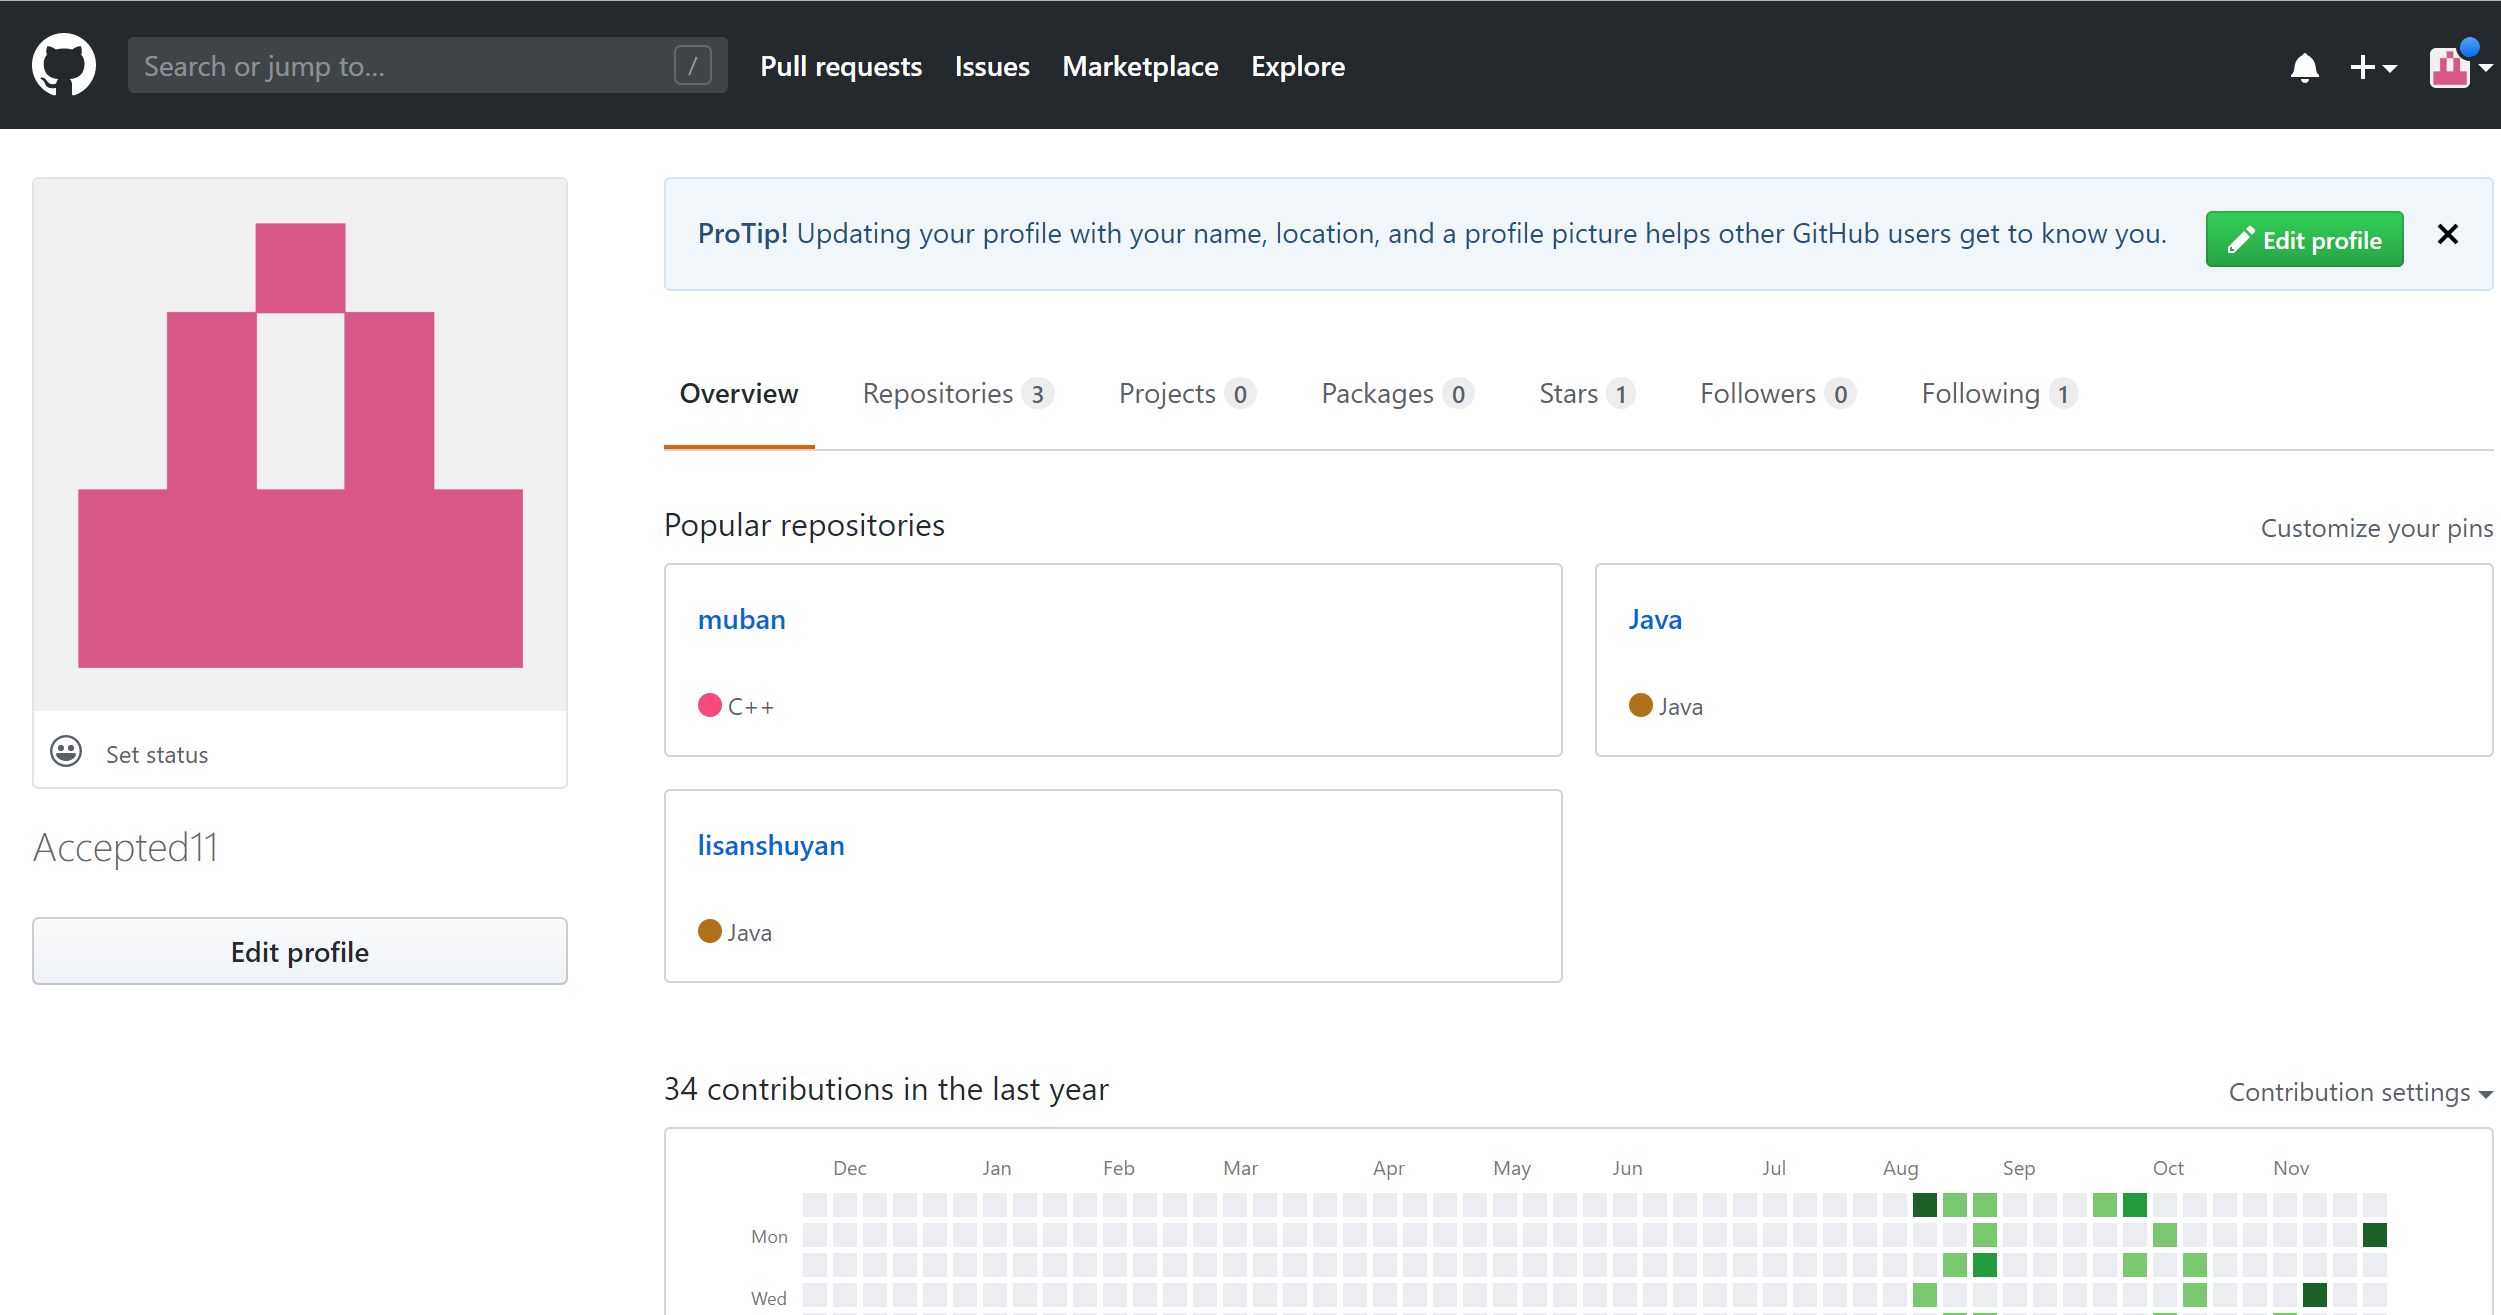
\includegraphics[width=12.5cm,height=5.5cm]{1.png}
                \caption{Github账户个人网站截图}
                \label{fig:universe}
            \end{figure}\\
    \item 观察者账户\\
          个人网址\\
          \url{https://user.guancha.cn/user/personal-homepage?uid=721877}\\
          个人网站截图
          \begin{figure}[h!]
                \centering
                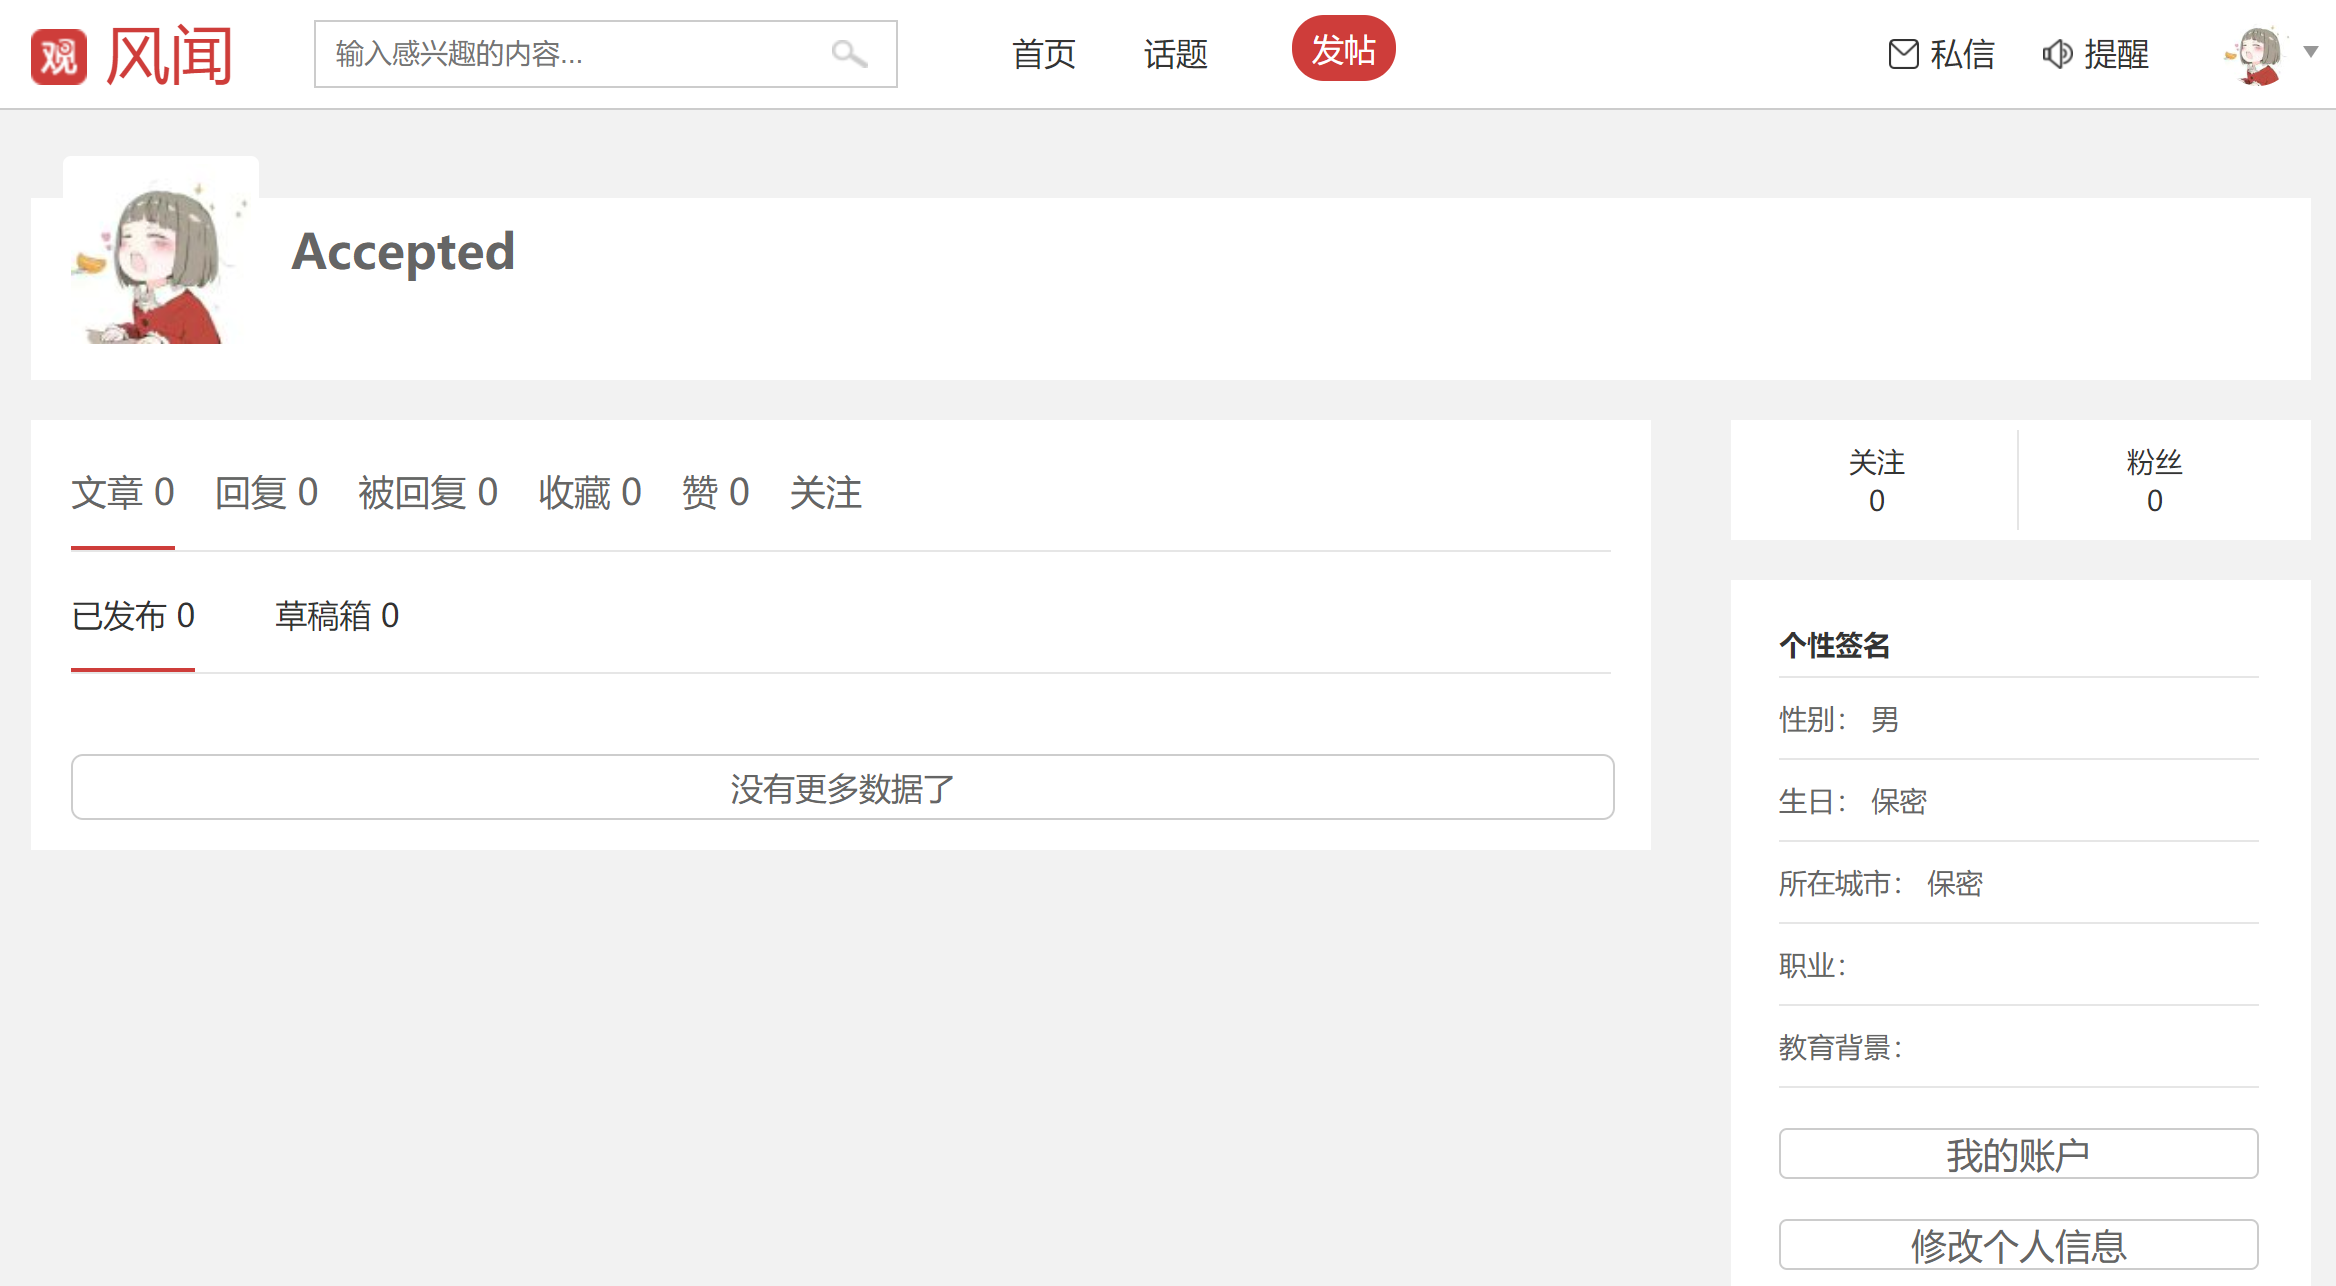
\includegraphics[width=12.5cm,height=5.5cm]{2.png}
                \caption{观察者账户个人网站截图}
                \label{fig:universe}
            \end{figure}
    \newpage
    \item 学习强国账户\\
          个人网址\\
          \url{https://pc.xuexi.cn/points/my-study.html}\\
          个人网站截图
          \begin{figure}[h!]
                \centering
                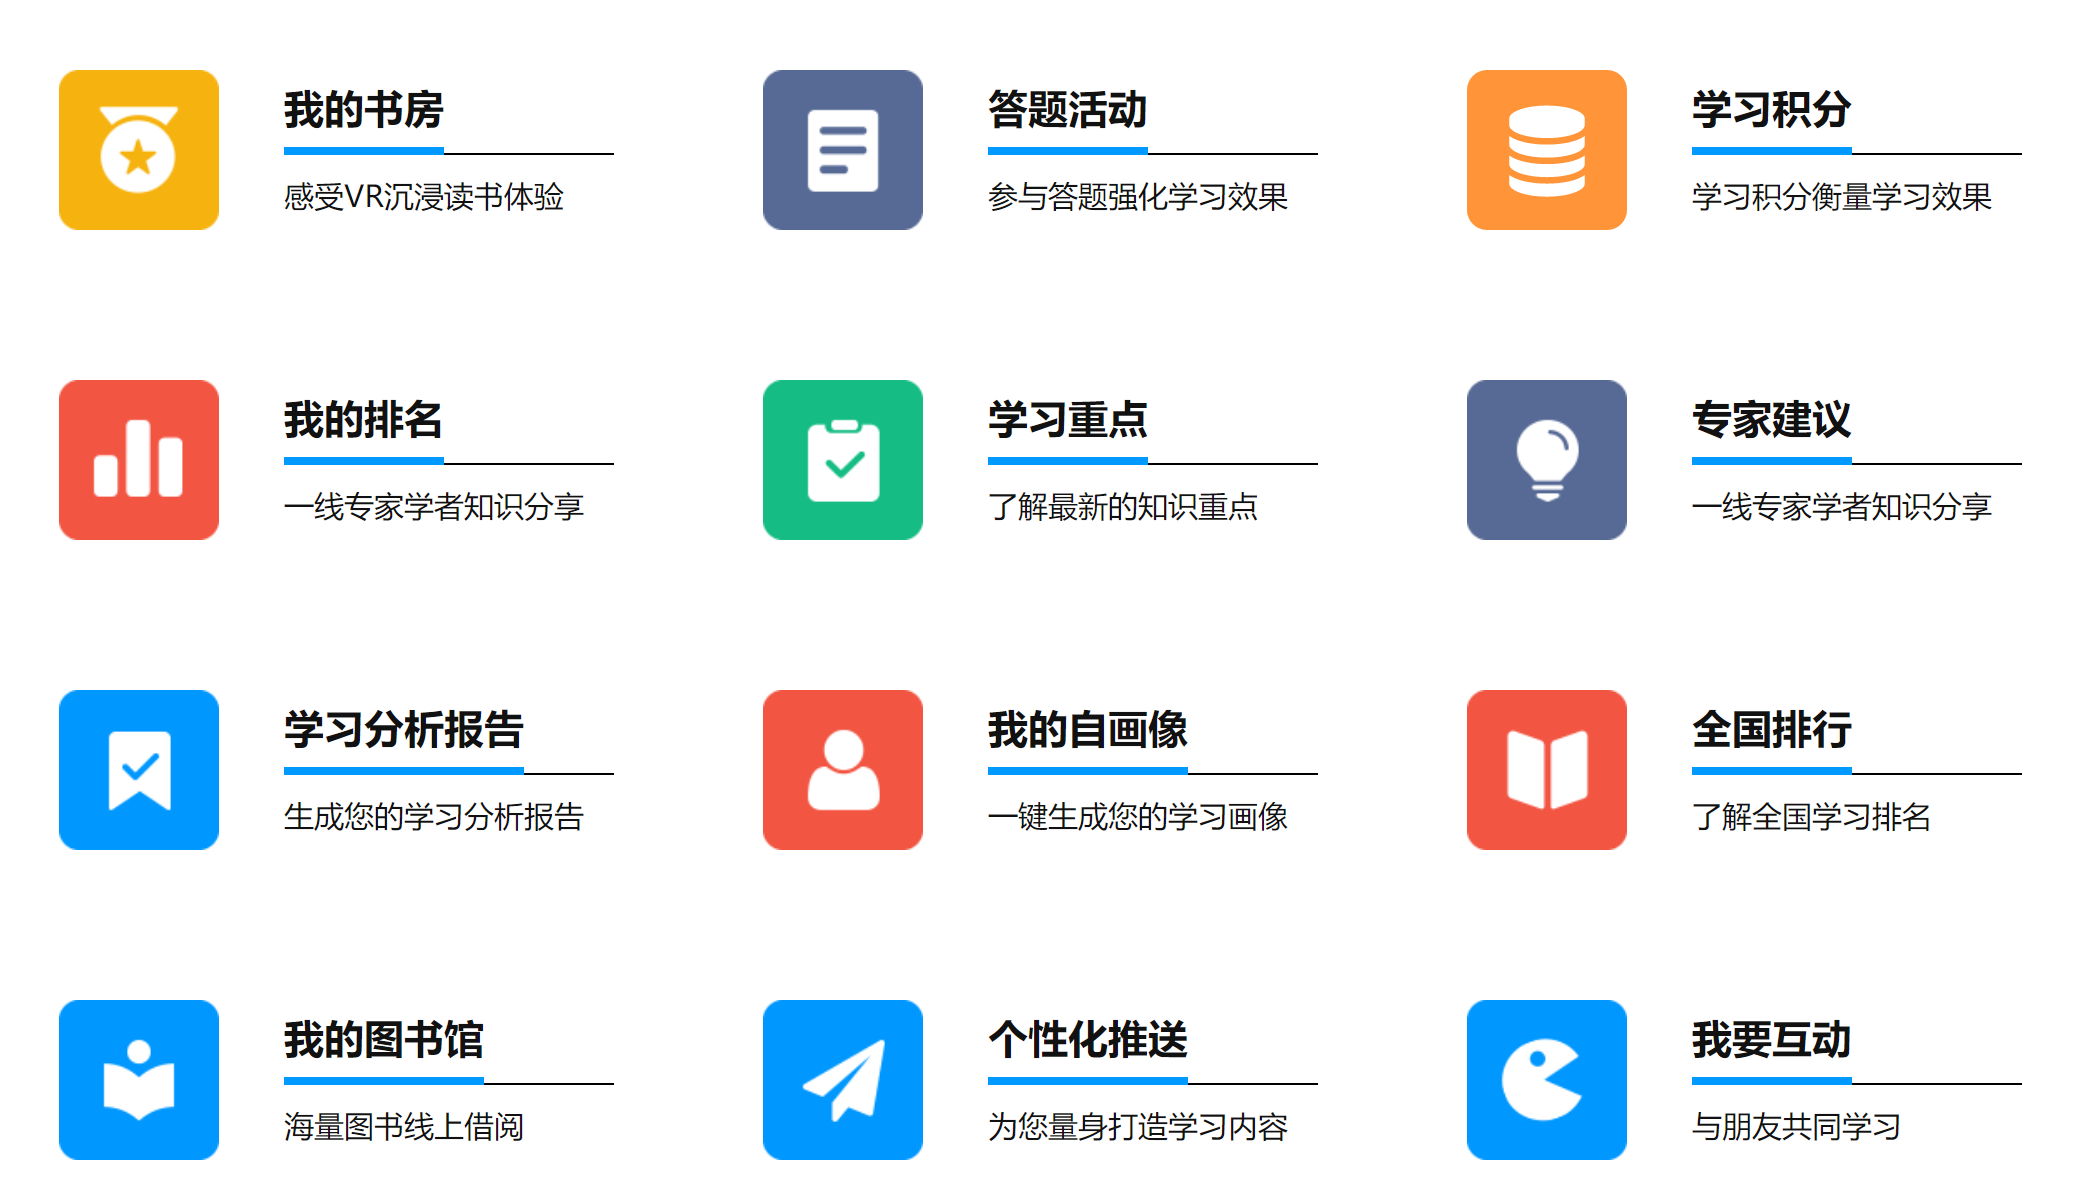
\includegraphics[width=12.5cm,height=5.5cm]{3.png}
                \caption{学习强国账户个人网站截图}
                \label{fig:universe}
            \end{figure}\\
    \item 哔哩哔哩APP\\
          个人网址\\
          \url{https://space.bilibili.com/391116115}\\
          个人网站截图
          \begin{figure}[h!]
                \centering
                
\includegraphics[width=12.5cm,height=5.5cm]{4.png}
                \caption{哔哩哔哩APP个人网站截图}
                \label{fig:universe}
            \end{figure}
    \newpage
    \item CSDN\\
          个人网址\\
          \url{https://blog.csdn.net/weixin_43601103}\\
          个人网站截图
          \begin{figure}[h!]
                \centering
                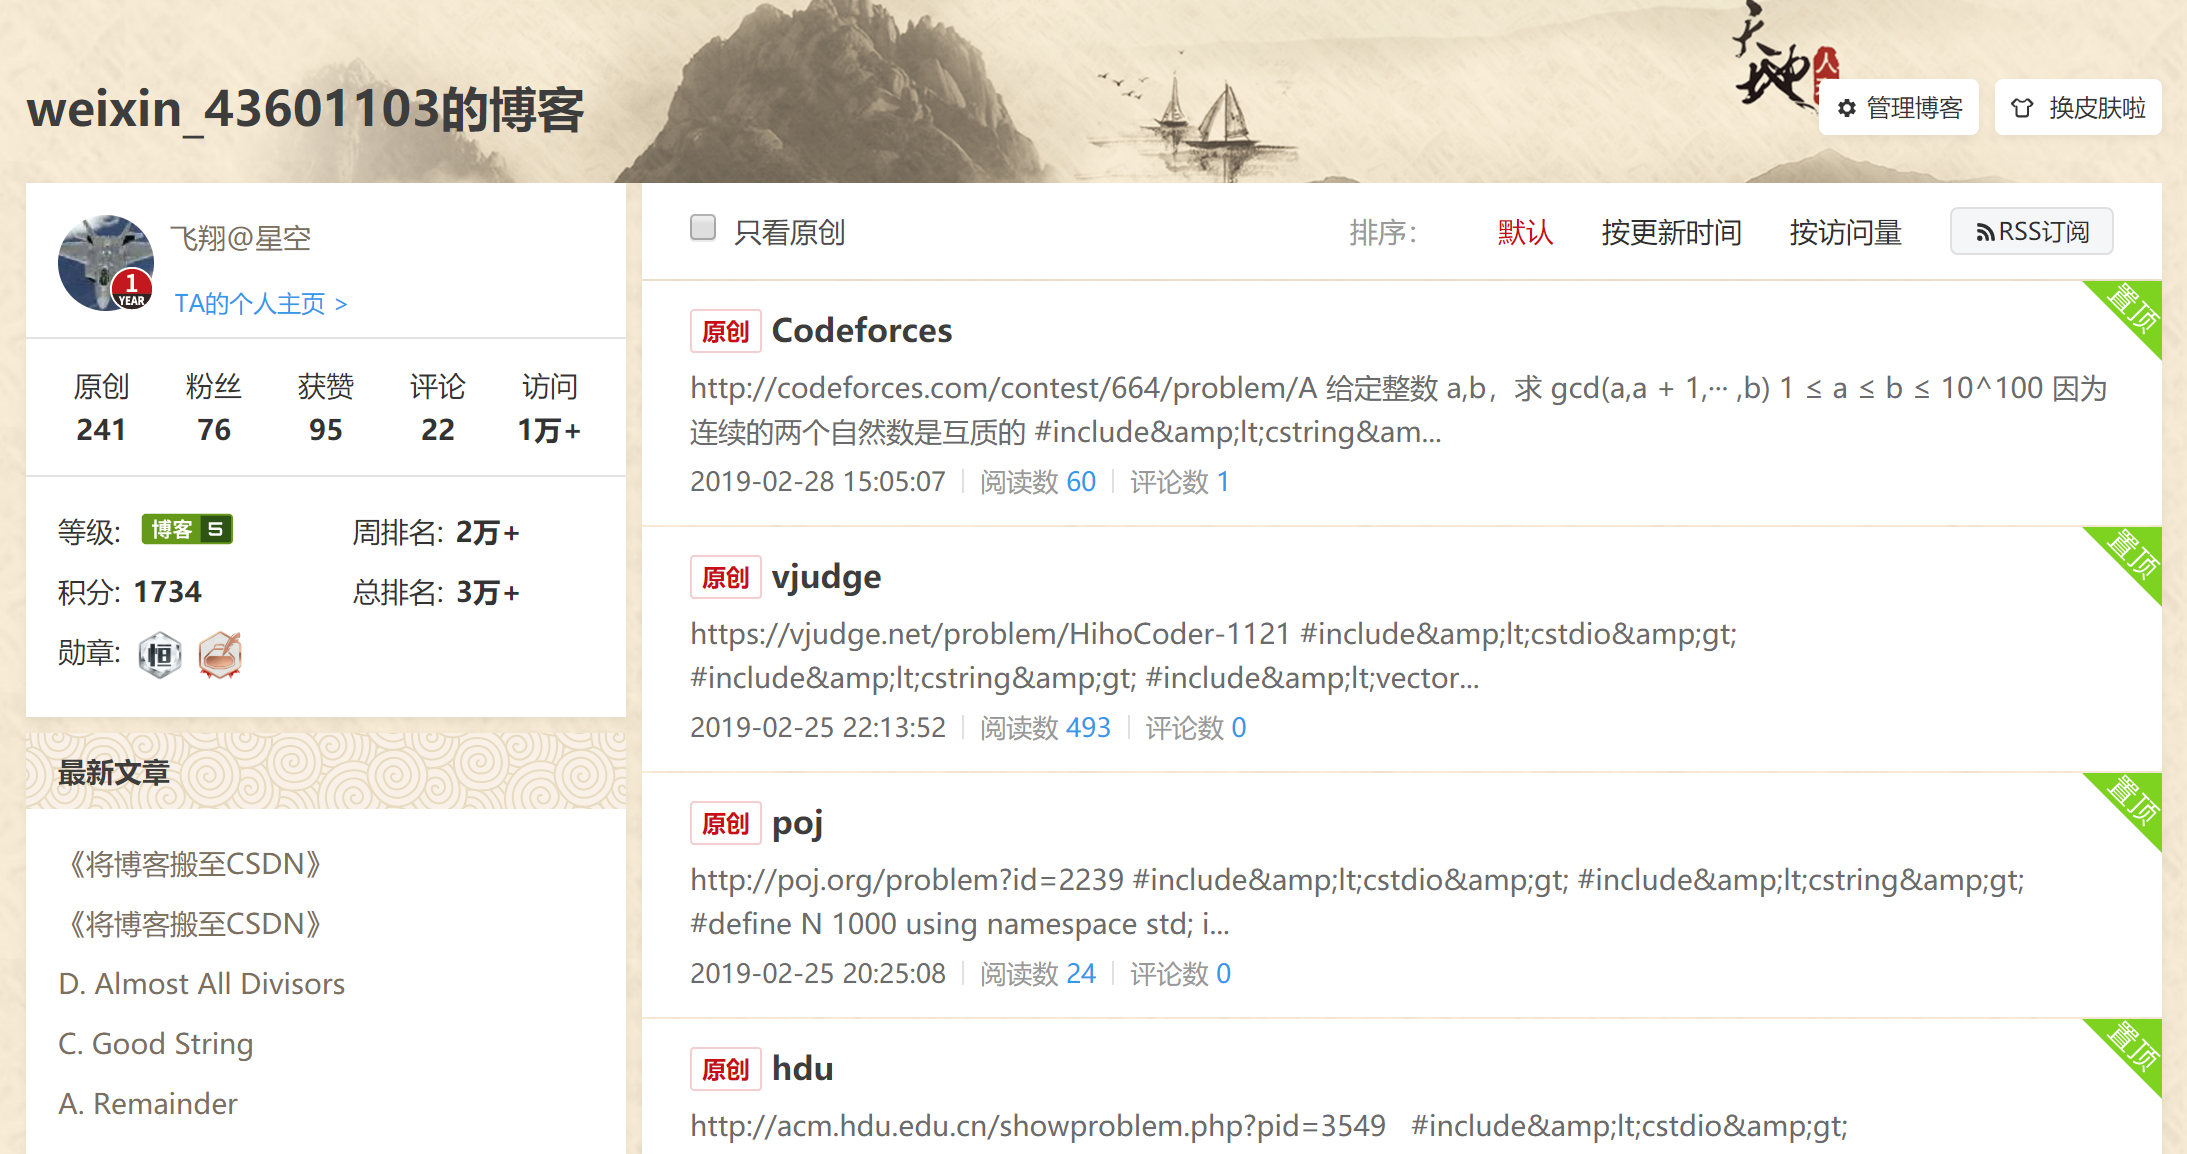
\includegraphics[width=12.5cm,height=5.5cm]{5.png}
                \caption{CSDN个人网站截图}
                \label{fig:universe}
            \end{figure}
    \item 博客园\\
          个人网址\\
          \url{https://www.cnblogs.com/Accpted/}\\
          个人网站截图
          \begin{figure}[h!]
                \centering
                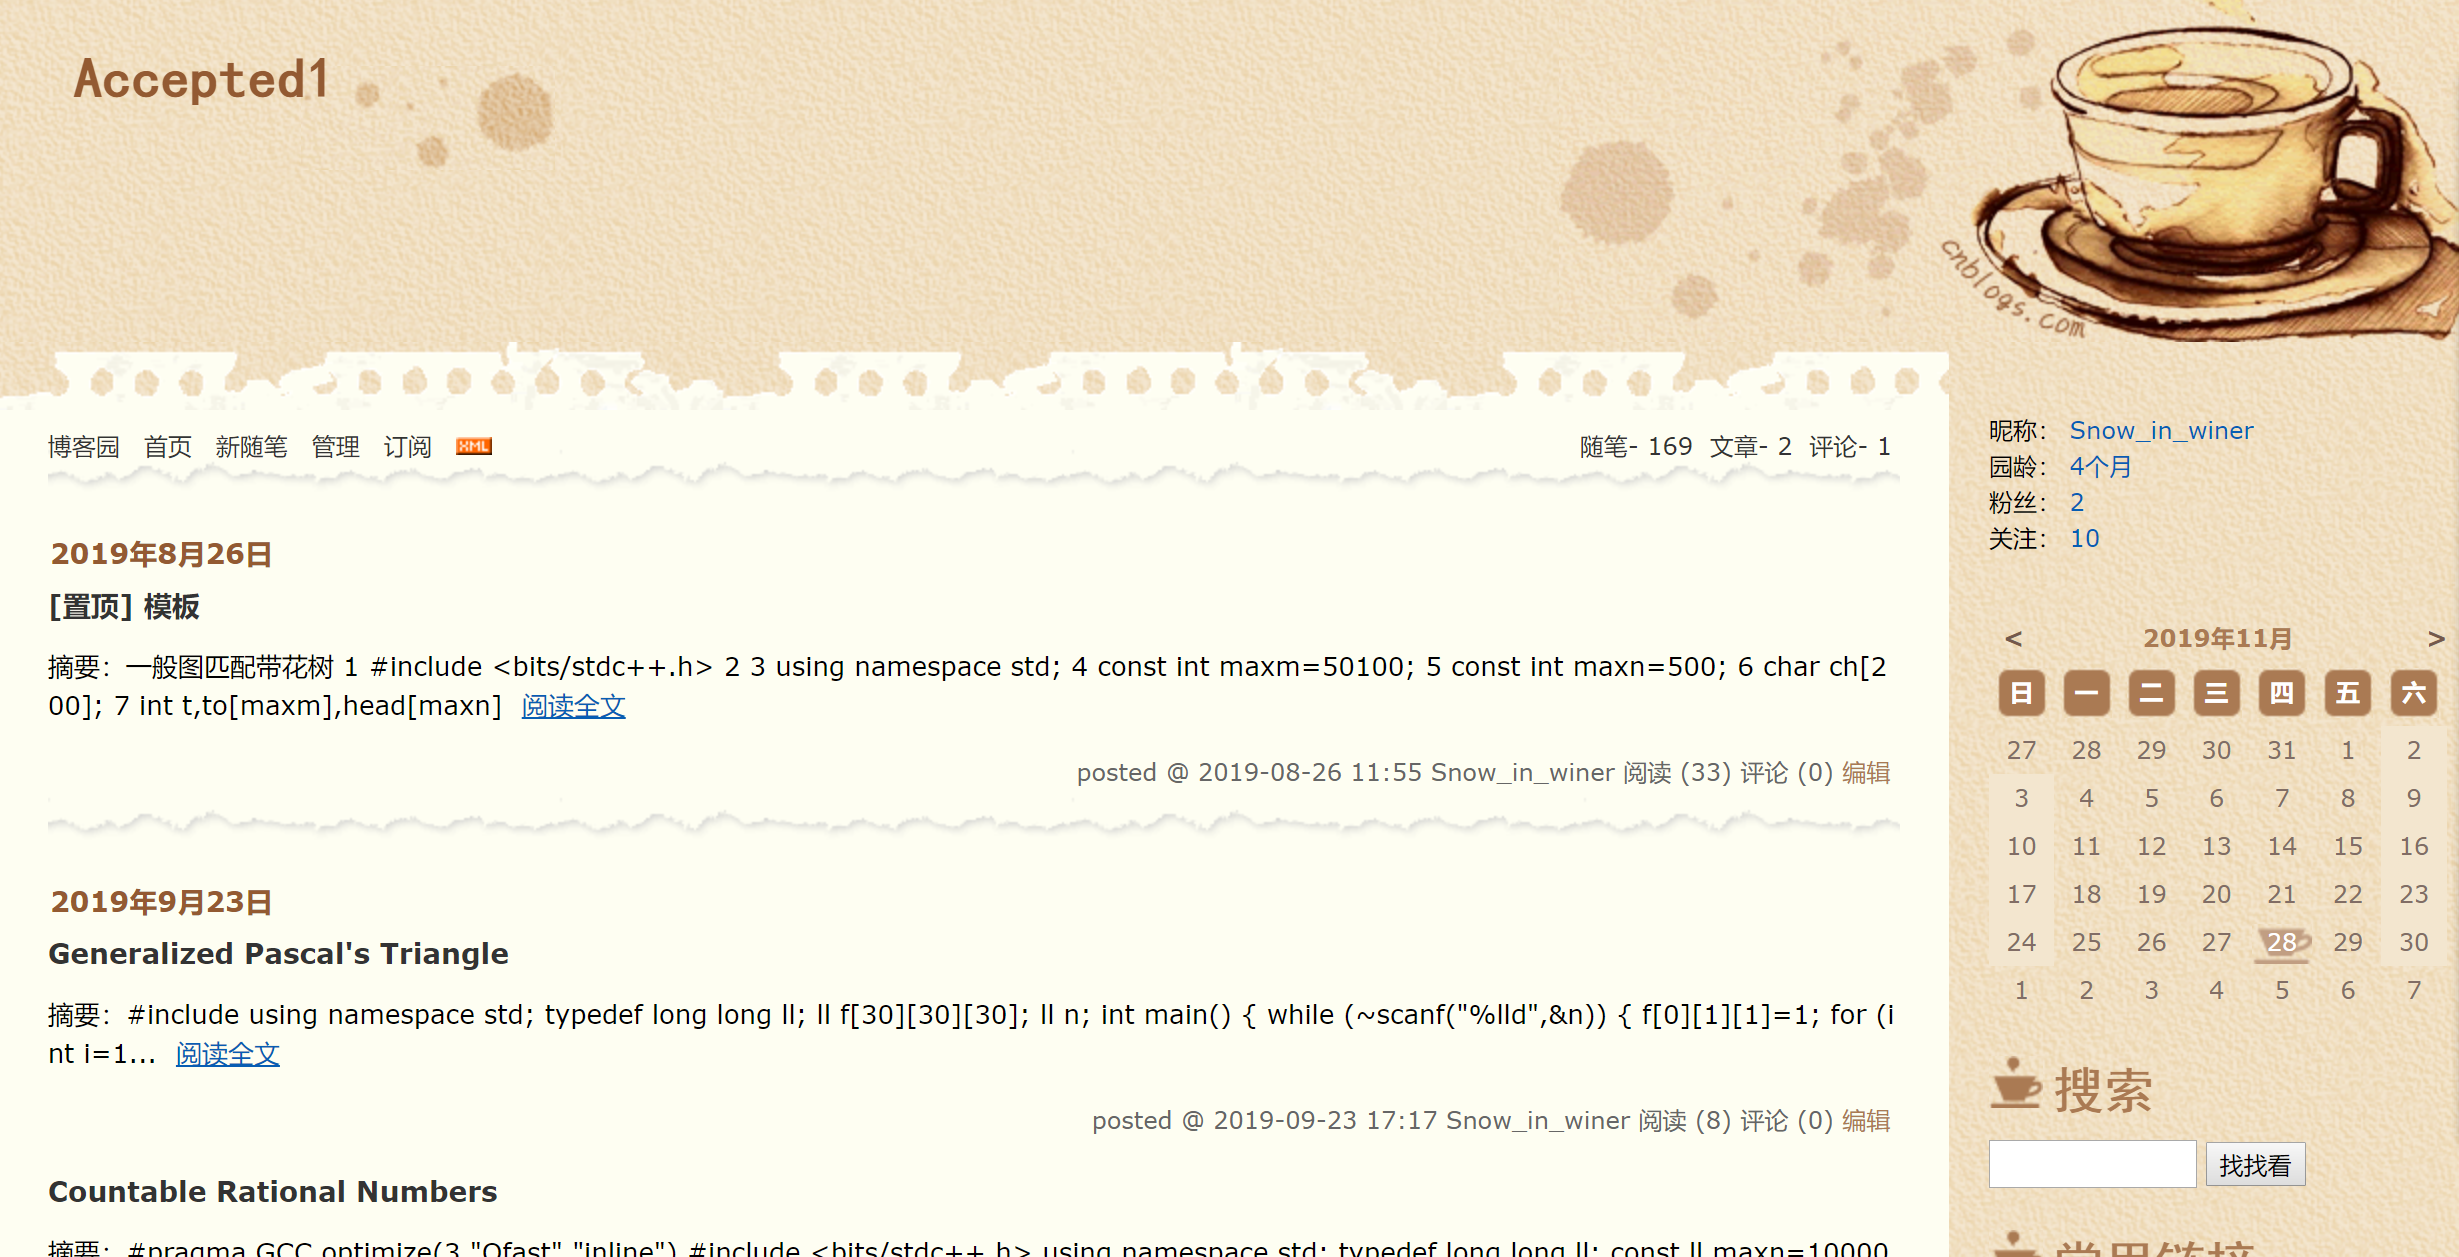
\includegraphics[width=12.5cm,height=5.5cm]{6.png}
                \caption{博客园个人网站截图}
                \label{fig:universe}
            \end{figure}
    \newpage
    \item 小木虫\\
          个人网址\\
          \url{http://muchong.com/bbs/space.php?uid=19953360}\\
          个人网站截图
          \begin{figure}[h!]
                \centering
                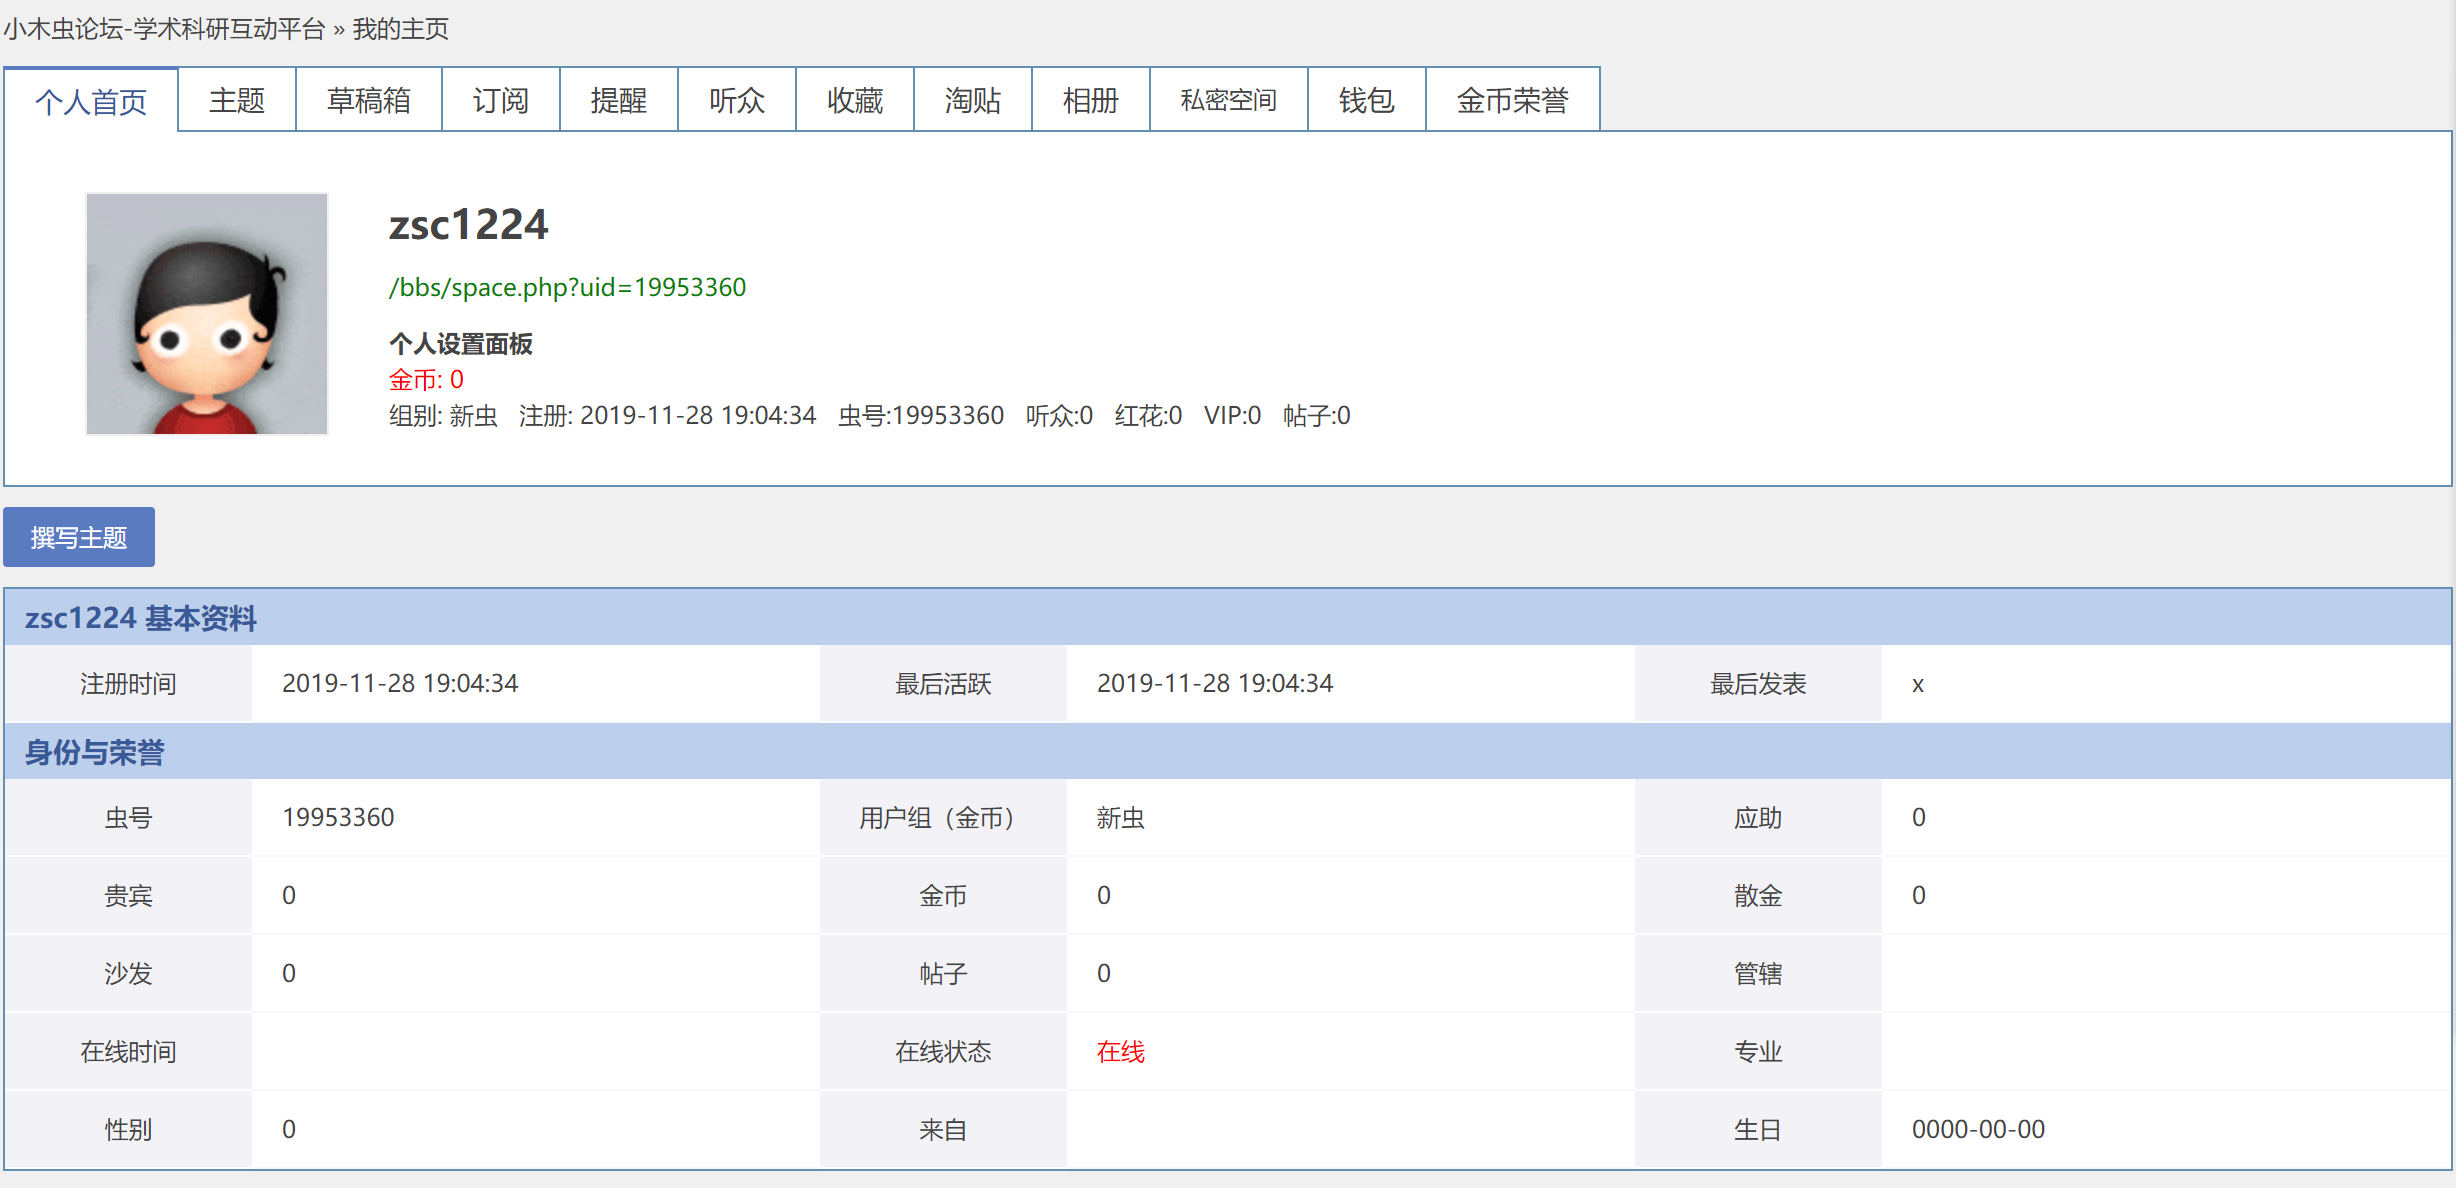
\includegraphics[width=12.5cm,height=5.5cm]{7.png}
                \caption{小木虫个人网站截图}
                \label{fig:universe}
            \end{figure}
\end{itemize}


\newpage
\hspace*{\fill} \\

\bibliographystyle{plain}
\bibliography{references}

\end{document}
